\label{sec:methdology}
In this section, we introduce the MetaFind, formalize the retrieval task, and present our dual-tower architecture with modality-aware fusion and the ESSGNN layout encoder. We describe the training strategy and the iterative scene composition process for contextually coherent 3D asset retrieval.
% \vspace{-0.05in}
\subsection{Task Definition}
% \vspace{-0.05in}
We aim to accurately retrieve contextually coherent 3D assets from a large-scale repository, given a user query and optional existing scene layout information. Formally, our retrieval task can be defined as follows: given an input query \( Q = \{q_{text}, q_{img}, q_{pc}, q_{layout}\} \), which may include text \(q_{text}\), images \(q_{img}\), 3D point clouds \(q_{pc}\), and optionally layout context \(q_{layout}\), the system retrieves the asset \(A^*\) from a pre-encoded asset database \(\mathcal{A}\):
\begin{equation}
    A^* = \arg\max_{A \in \mathcal{A}} \text{sim}(f_{query}(Q), f_{gallery}(A)),
\end{equation}
where $f_{query}$ and $f_{gallery}$ represent the query and gallery encoders, and $\text{sim}(\cdot, \cdot)$ denotes the similarity function. The task is challenging due to the multimodal nature of user queries, partial modality absence, and the necessity for accurate layout awareness to ensure spatial coherence and realism.
% \vspace{-0.05in}
\subsection{Method Overview}
% \vspace{-0.05in}
To address the above challenge, we introduce MetaFind, as shown in \ref{fig:framework}, a dual-tower retrieval framework consisting of a query encoder and a gallery encoder, both leveraging the ULIP-2 embedding backbone. The gallery encoder precomputes embeddings for assets using three available modalities, which are then stored for efficient retrieval. On the query side, the encoder is designed to flexibly handle arbitrary combinations of modalities and, optionally, layout information—accommodating partial modality absence through a modality-aware fusion strategy. Specifically, each available modality is independently encoded using the ULIP-2 backbone, and these modality embeddings are subsequently integrated via a fusion layer, such as mean pooling, an MLP, or a Transformer-based module, generating a unified representation. Furthermore, the query encoder optionally integrates a layout encoder (ESSGNN) to capture spatial context from the existing scene layout. The layout is modeled as a structured graph with nodes representing placed objects (each described by spatial coordinates and semantic embeddings) and edges capturing spatial relationships. The layout encoder processes this graph to produce a context-aware layout vector, enhancing the spatial reasoning capability of the retrieval process. Its equivariant property ensure stable and generalizable scene embeddings under varying coordinate frames and unnormalized layouts common in open-world environments. 

Our training protocol involves two stages: First, we train the query and gallery encoders to learn fundamental multimodal embedding alignment without spatial context. Subsequently, we fine-tune the query encoder—particularly the fusion module and the layout encoder—using layout-aware room-level datasets. This fine-tuning stage employs adaptive freezing strategies, selectively freezing components like the gallery encoder to balance performance and computational efficiency.
% \vspace{-0.05in}
 \subsection{Data Preparation}
 % \vspace{-0.05in}
\begin{figure}[t]
    \centering
    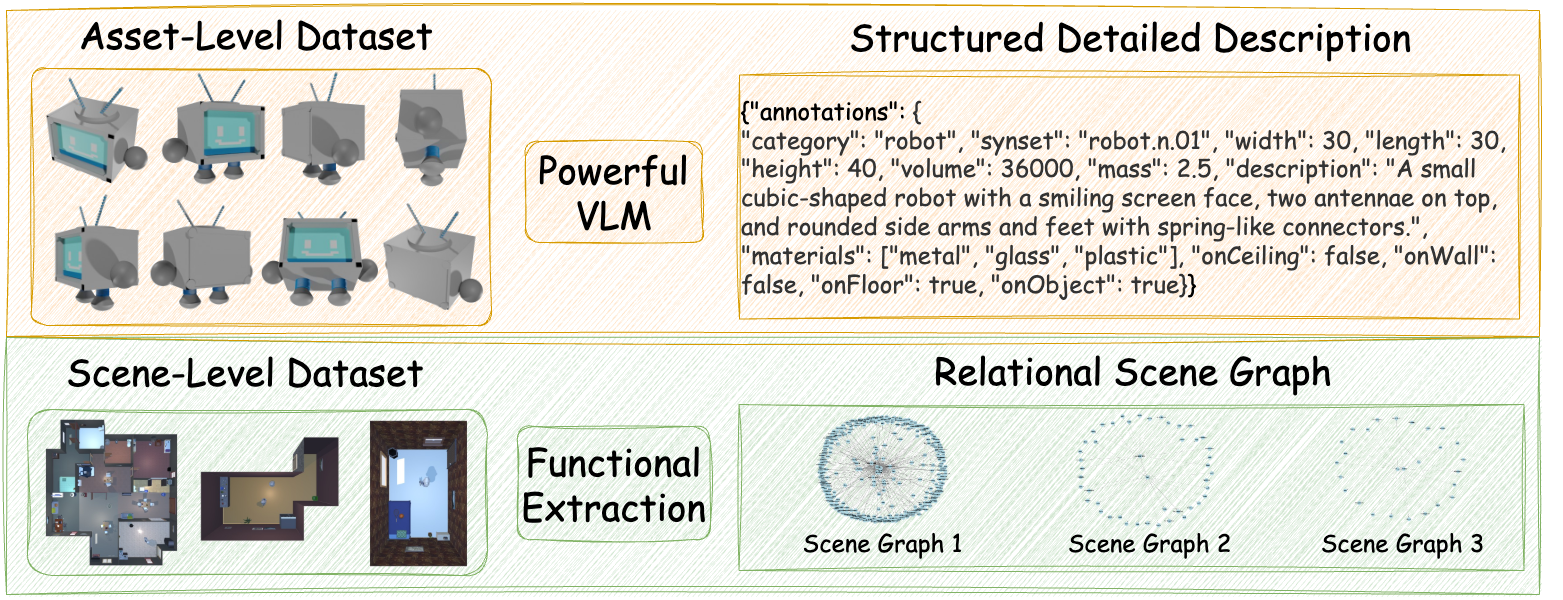
\includegraphics[width=1\linewidth]{data-preprocess.png}
    % \vspace{-0.25in}
    \caption{Data preparation pipeline. At the asset level (top), each 3D object from Objaverse-LVIS is rendered from multiple orthogonal views and passed through a VLM to generate structured, detailed annotations, capturing attributes such as category, dimensions, materials, and spatial placement constraints. At the scene-level (bottom), functional extraction is performed on generated rooms from the ProcTHOR, resulting in relational scene graphs encoding the spatial and semantic relationships between placed objects, enabling layout-aware retrieval capabilities in MetaFind.}
    \label{fig:data-sample}
    % \vspace{-0.2in}
\end{figure}
Our methodology requires prepared datasets at both object and scene levels to support multimodal and layout-aware retrieval tasks (as illustrated in Figure \ref{fig:data-sample}). For object-level representation learning, we utilize the Objaverse-LVIS dataset, which comprises approximately 48,000 distinct 3D assets. Each asset is rendered from 11 orthogonal viewpoints and annotated using GPT-4o. These annotations provide rich textual descriptions detailing attributes such as object category, size dimensions, materials, and placement constraints. For scene-level data, we leverage the ProcTHOR, which includes over 10,000 generated houses constructed from a curated collection of more than 3,000 unique assets. Each room configuration provides precise spatial coordinates and comprehensive semantic metadata for each asset, enabling the extraction of structured graphs representing object-level placements and spatial relationships. The bottom side of Figure \ref{fig:data-sample} illustrates the extraction process of such structured scene graphs. These graphs form the basis for training the layout-aware ESSGNN encoder, effectively capturing spatial coherence and relational context crucial for accurate asset retrieval. They include two types of edges: (i) physical-relation edges that capture spatial dependencies (e.g., “cup on table”); and (ii) semantic-relation edges that capture functional or contextual associations (e.g., “microscope–lab bench”), obtained by prompting an LLM on object pairs. This dual-edge design encodes both physical layout and high-level semantics, enhancing retrieval and layout reasoning.
% \vspace{-0.05in}
\subsection{Dual-Tower Architecture and Fusion Design}
% \vspace{-0.05in}
While prior works typically align 3D encoders to a fixed CLIP embedding space by freezing pretrained text and image encoders, our MetaFind framework adopts a more flexible dual-tower design. It enables context-aware, multi-modal queries by training a dedicated query encoder that fuses arbitrary modality subsets—including text, image, and scene-aware 3D inputs.

MetaFind employs a dual-tower architecture with separate encoders for the query and gallery. Each tower leverages ULIP-2 to independently encode available modalities (text, images, and point clouds). A modality-aware fusion module combines these modality embeddings via one of several strategies, such as mean pooling, MLP, masked MLP, gated fusion, or Transformer-based fusion. The gallery encoder is modality-complete and frozen after pretraining, while the query encoder remains flexible: It accepts any subset of modalities and can be augmented with a layout-aware vector. This vector is extracted using our proposed Equivariant Spatial-Semantic Graph Neural Network (ESSGNN) trained on scene graphs, enabling the model to incorporate spatial context for scene-aware retrieval.
% \vspace{-0.05in}
\subsection{ESSGNN: Scene-Aware Equivariant Graph Encoder}
% \vspace{-0.05in}
In this work, we propose the \textbf{Equivariant Spatial-Semantic Graph Neural Network (ESSGNN)} to encode 3D scene layouts in a way that is both spatially grounded and semantically expressive. ESSGNN is designed to maintain equivariance to SE(3) transformations during message passing while incorporating semantic relationships between objects through learned edge representations.

We initially experimented with standard Graph Attention Networks (GATs) to model inter-object dependencies based on spatial adjacency. However, we observed that GATs were highly sensitive to global translation and scaling variations across scenes, resulting in unstable layout embeddings and poor generalization. These issues are especially prominent in open-world or metaverse environments, where object positions are defined in large and often unnormalized coordinate systems, with no guarantee that scenes are aligned or centered.

Motivated by recent advances in drug design—where Equivariant Graph Neural Networks (EGNNs \cite{satorras2021n}) have been effectively applied to model 3D molecular structures invariant to spatial transformations—we design ESSGNN to address these limitations. Our model extends the EGNN formulation to incorporate semantic edge features in addition to geometric ones, allowing message passing to be informed not only by spatial proximity but also by functional or compositional relationships between objects. Given a scene graph \( G = (\mathcal{V}, \mathcal{E}) \), each node \( v_i \in \mathcal{V} \) represents an object with 3D position \( x_i \in \mathbb{R}^3 \) and a text-derived feature \( t_i \in \mathbb{R}^d \). The node feature is initialized as:
\[
    h_i^{(0)} = \text{Concat}(x_i, t_i).
\]

Edges in the graph include both spatial and semantic relationships. Spatial edges are extracted from physical layout constraints (e.g., adjacency, support), while semantic edges are generated by prompting a large language model (LLM) with object descriptions to produce natural language relation sentences. These sentences are then encoded into dense vectors using a frozen text encoder (e.g., CLIP or BERT), resulting in edge embeddings \( e_{ij} \) that carry functional and relational meaning.

The message-passing mechanism in ESSGNN follows a modified Equivariant Graph Convolutional Layer (EGCL) structure. For each layer \( l \), node features and positions are updated as:
\begin{align}
    h_i^{l+1} &= h_i^l + \sum_{j \in \mathcal{N}(i)} f_h(d_{ij}^l, h_i^l, h_j^l, e_{ij}; \theta_h), \\
    x_i^{l+1} &= x_i^l + \sum_{j \in \mathcal{N}(i)} (x_i^l - x_j^l) \cdot f_x(d_{ij}^l, h_i^{l+1}, h_j^{l+1}, e_{ij}; \theta_x),
\end{align}
where \( d_{ij}^l = \|x_i^l - x_j^l\|_2 \) is the Euclidean distance between nodes, and \( f_h: \mathbb{R}^{(2d + 1 + e)} \to \mathbb{R}^d \), \( f_x: \mathbb{R}^{(2d + 1 + e)} \to \mathbb{R}^{3} \) are two learnable functions parameterized by \( \theta_h \) and \( \theta_x \), respectively, which we approximate using multilayer perceptrons (MLPs). Here, \( e \) denotes the dimension of the semantic edge embedding \( e_{ij} \). After \( L \) layers, the node features are aggregated into a global layout embedding:
\[
    e_{\text{layout}} = \text{Pooling}(\{h_i^{(L)}\}).
\]

This embedding is integrated into the query encoder of our dual-tower retrieval framework to provide scene-aware conditioning. ESSGNN generalizes the original EGNN by introducing \textit{semantic-aware edge modulation}, enabling it to operate on multi-relational graphs with heterogeneous object types and to better handle complex spatial-functional layouts found in real-world and virtual 3D scenes.

Our model retains full SE(3)-equivariance concerning input transformations. Specifically, for any rotation operator \( R \in SO(3) \) and translation vector \( T \in \mathbb{R}^3 \), the following condition holds:
\begin{align}
    (R x^{l+1} + T,\, h^{l+1}) = \text{ESSGNN}(R x^l + T,\, h^l,\, E). \label{eq:EGCL_equivariance}
\end{align}
We provide a formal proof of this equivariance property in Appendix~\ref{sec:appendix_equiv_proof}, extending the original EGCL proof to include semantic edge features.


% \vspace{-0.05in}
\subsection{Training Strategy}
% \vspace{-0.05in}
We adopt a two-stage training strategy that aligns with the dual-tower architecture and the flexible, multimodal nature of the retrieval task. In the first stage, we focus on learning robust cross-modal representations that can handle arbitrary combinations of query modalities. In the second stage, we incorporate scene layout information through an ESSGNN encoder, enabling the system to perform context-aware retrieval grounded in spatial reasoning.
% \vspace{-0.1in}
\subsubsection*{Stage 1: Cross-Modal Alignment Pretraining.}
% \vspace{-0.05in}
In the first stage, both query and gallery encoders are trained on large-scale object-level data from Objaverse-LVIS, where each asset has full modality inputs (text, images, and point clouds). We introduce stochastic modality masking to simulate partial-modality queries: each modality in the query has a 30\% probability of being independently masked. Rather than zero-padding, we apply masked embeddings to ensure flexibility and prevent model degradation. The goal is to align all available modality combinations into a shared embedding space. The gallery encoder is trained to be modality-complete, and both towers share the contrastive retrieval objective:
\begin{equation}
    \mathcal{L}_{\text{pre}} = -\log \frac{\exp(\text{sim}(f_{\text{query}}(Q), f_{\text{gallery}}(A)) / \tau)}{\sum_{A' \in \mathcal{B}} \exp(\text{sim}(f_{\text{query}}(Q), f_{\text{gallery}}(A')) / \tau)},
\end{equation}
where \( \tau \) is a temperature hyperparameter and \( \mathcal{B} \) denotes the gallery batch. 
% \vspace{-0.1in}
\subsubsection*{Stage 2: Layout-Aware Fine-Tuning}
% \vspace{-0.05in}
In the second training stage, we enhance the query encoder with spatial context derived from the current scene layout. Given available modality embeddings for text \(e_{\text{text}}\), image \(e_{\text{img}}\), and point cloud \(e_{\text{pc}}\), along with the optional layout embedding \(e_{\text{layout}}\) produced by the ESSGNN module, the final fused query representation is computed as:
\begin{equation}
    e_{\text{query}} = \text{Fusion}(e_{\text{text}}, e_{\text{img}}, e_{\text{pc}}) + \lambda \cdot e_{\text{layout}},
\end{equation}
where \(\lambda\) is a learnable scalar controlling the contribution of layout information. This residual design allows layout reasoning to enhance retrieval without disrupting the original embedding space.

To ensure robustness in real-world settings where scene layouts may not always be available, we introduce \textit{stochastic scene dropout} during training: the layout vector \(e_{\text{layout}}\) is omitted in 30\% of batches, forcing the model to generalize to layout-free inputs. Only the query-side fusion layer and the ESSGNN module are updated during this stage; the gallery encoder is frozen to reduce training costs and preserve asset embedding consistency.

We adopt a \textbf{bidirectional contrastive learning} objective to symmetrically align query and gallery embeddings. Let \(e_{\text{query}}\) and \(e_{\text{gallery}}\) denote the fused query and gallery embeddings, respectively. The layout-aware retrieval loss is defined as:
{\small
\begin{equation}
    \mathcal{L}_{\text{layout}}^{\text{q2g}} = -\log \frac{\exp(\text{sim}(e_{\text{query}}, e_{\text{gallery}}) / \tau)}{\sum_{e'_{\text{gallery}} \in \mathcal{B}} \exp(\text{sim}(e_{\text{query}}, e'_{\text{gallery}}) / \tau)}, \quad
    \mathcal{L}_{\text{layout}}^{\text{g2q}} = -\log \frac{\exp(\text{sim}(e_{\text{gallery}}, e_{\text{query}}) / \tau)}{\sum_{e'_{\text{query}} \in \mathcal{B}} \exp(\text{sim}(e_{\text{gallery}}, e'_{\text{query}}) / \tau)}
\end{equation}
}

where \(\tau\) is a temperature hyperparameter, and \(\mathcal{B}\) denotes the batch of negatives. The final loss is the average of the two directions:
\begin{equation}
    \mathcal{L}_{\text{layout}} = \frac{1}{2} \left( \mathcal{L}_{\text{layout}}^{\text{q2g}} + \mathcal{L}_{\text{layout}}^{\text{g2q}} \right).
\end{equation}

This training strategy encourages accurate retrieval of relevant assets (query-to-gallery) and consistent representation of assets retrievable by matching scene context (gallery-to-query). The model improves generalization and robustness by aligning both directions, especially in iterative scene construction where queries and context evolve.



% \vspace{-0.05in}
\subsection{Inference and Iterative Composition}
% \vspace{-0.05in}
At inference time, all gallery asset embeddings are precomputed and cached for efficient retrieval. Given an input query—which may consist of any combination of text, image, point cloud, and optional scene layout—the query encoder generates a layout-aware embedding used to identify the most contextually suitable asset from the gallery. 

To construct complete scenes, we deploy an iterative composition strategy shown in Algorithm~\ref{alg:iterative}. Instead of retrieving all required objects independently in a single step, we retrieve and place one object at a time. After each placement, the scene graph is updated to reflect the new layout, and the ESSGNN module recomputes the layout embedding, allowing subsequent retrievals to account for the evolving spatial context. While this step-by-step process introduces additional computational latency compared to one-shot parallel retrieval, it significantly improves spatial coherence and contextual alignment across placed objects, resulting in more realistic and visually harmonious scenes.

\textbf{Efficiency considerations.} The iterative pipeline incurs extra latency and compute versus one-shot retrieval—especially for multi-object scenes—but this trade-off is use-case dependent and tunable. When global coherence and stylistic consistency matter most, a fully sequential schedule yields the best quality. When efficiency is prioritized, we use parallel retrieval or region-based decomposition: partition a room into semantic/spatial regions (e.g., seating, storage), retrieve sequentially within each region to preserve local coherence, and process regions in parallel to improve throughput. This design flexibility makes the method practical across scenarios, and we have clarified it in the revision.

\begin{algorithm}[t]
\caption{Iterative Layout-Aware Scene Composition}
\label{alg:iterative}
\begin{algorithmic}[1]
\REQUIRE Precomputed gallery embeddings $\mathcal{E}_{\text{gallery}}$, initial scene graph $G_0$, asset query list $\{Q_1, Q_2, ..., Q_N\}$

\STATE Initialize scene graph $G \leftarrow G_0$

\FOR{$i = 1$ to $N$}
    \STATE Extract current layout embedding: $e_{\text{layout}} \leftarrow \text{EGNN}(G)$
    \STATE Encode available modalities of query $Q_i$: $e_{\text{text}}, e_{\text{img}}, e_{\text{pc}}$
    \STATE Fuse into layout-aware query: $e_{\text{query}} \leftarrow \text{Fusion}(e_{\text{text}}, e_{\text{img}}, e_{\text{pc}}) + \lambda \cdot e_{\text{layout}}$
    \STATE Retrieve best-matching asset: $A^*_i \leftarrow \arg\max_{A \in \mathcal{E}_{\text{gallery}}} \text{sim}(e_{\text{query}}, e_{\text{gallery}}(A))$
    \STATE Place $A^*_i$ into the scene, update scene graph: $G \leftarrow G \cup \{A^*_i\}$
\ENDFOR

\STATE \textbf{return} Final composed scene $G$
\end{algorithmic}
\end{algorithm}